\documentclass[conference]{IEEEtran}
\usepackage[utf8]{inputenc}
\usepackage{cite}
\usepackage{amsmath,amssymb,amsfonts}
\usepackage{algorithmic}
\usepackage{graphicx}
\usepackage{textcomp}
\usepackage{xcolor}

%Added 
\graphicspath{ {./images/} }
\usepackage{stfloats}
\usepackage[all]{nowidow} \setnoclub

\def\BibTeX{{\rm B\kern-.05em{\sc i\kern-.025em b}\kern-.08em
    T\kern-.1667em\lower.7ex\hbox{E}\kern-.125emX}}
\begin{document}

\title{AlphaGo: an Atypical Go program}

% \author{\IEEEauthorblockN{1\textsuperscript{st} Given Name Surname}
% \IEEEauthorblockA{\textit{dept. name of organization (of Aff.)} \\
% \textit{name of organization (of Aff.)}\\
% City, Country \\
% email address or ORCID}
% }

\author{\IEEEauthorblockN{Shubham Kamble}
\IEEEauthorblockA{
% \textit{Institut für Data Science im Maschinenbau} \\
\textit{Rheinisch-Westfälische Technische Hochschule Aachen}\\
Aachen, Germany \\
shubham.kamble@rwth-aachen.de}
}

% {}^2 \textit{Intelligent Control Systems Group, Max Planck Institute for Intelligent Systems, solowjow@is.mpg.de}
% \textsuperscript{1},
% Friedrich Solowjow\textsuperscript{2}

\maketitle

\begin{abstract}
The game of Go has challenged artificial intelligence researchers for many decades. One of the reasons is its enormous search space, which makes it challenging to find the optimal policy. Additionally, there are only few heuristics to evaluate a board position (to determine who is winning). Thus, rewards become sparse. However, a new paradigm for search, based on Monte-Carlo simulation combined with deep convolutional neural networks, has revolutionized the state-of-the-art. Nowadays, they can play at human-master levels and win in time-control games. Here, we discuss this search approach that uses `policy networks' to select moves and `value networks' to evaluate board positions trained using a reinforcement learning framework. Further, an asynchronous policy and value Monte Carlo tree search algorithm combines these networks that initially achieved a playing strength sufficient to defeat the best human players. Finally, the analysis of this new search approach has unraveled new AI techniques for general computer game-playing.
\end{abstract}

\begin{IEEEkeywords}
artificial intelligence, Monte Carlo simulation, deep reinforcement learning, computer Go
\end{IEEEkeywords}

\section{Introduction}
Sequential decision-making is one of the fundamental problems of artificial intelligence (AI). The challenge is to get an agent to select a sequence of actions that maximizes a long-term objective (e.g., winning a game). Planning and search have been widely applied to solve such problems \cite{b1}. Planning is the computation process by which the agent updates its action selection policy $\pi(s_t, a_t)$, where $s_t \in S$ and $a_t \in A$ are state and action taken in state $s_t$ at time-step $t$, respectively. Search refers to the computation process used to select an action from a particular root state $s_0 \in S$. We adopt the definition of planning used typically in reinforcement learning \cite[pp.~1--11]{b2} and the definition of search often used in two-player games \cite[pp.~192--203]{b3}.

Game-playing research is interesting and essential for the AI community\cite{b4}. The reason is generally twofold: first, games provide cheap, reproducible environments suitable for testing new search algorithms, pattern-based evaluation methods, or learning concept, second, there is a \textit{human aspect} of artificial game playing: people like to challenge themselves (by machines) in their mental abilities. 
%This \textit{psychological layer} of a human-machine competition is crucial and cannot be overestimated. 
In this rivalry, the machines have already surpassed the top human players in several challenging games.

Classic two-player and perfect information games have been used as excellent testbeds. In games such as chess\cite{b5}, checkers\cite{b6}, Othello\cite{b7}, and backgammon\cite{b8}, human performance levels have been exceeded by programs that combine brute force tree-search\cite{b9} with human knowledge or reinforcement learning. However, before 2015, these approaches and others have failed to achieve equivalent performance in the game of Go, mainly due to its enormous search space. Furthermore, simple heuristics for evaluating the position, like those proven to be successful in chess, are hard to design for Go\cite{b10}. Also, there are long-term influences of the moves that affect the outcome of the game hundreds of moves later. Therefore, a Go program that must simultaneously cope with the enormous game complexity, long-term effects of moves and evaluate the strategic importance of positions posed a grand challenge. Hence, progress in computer Go was thought to ultimately contribute to advancing the field of AI as a whole\cite{b11}.

Silver et al.\cite{b12} have shown that two general principles can reduce this effective search space: reducing the depth, $d$, using a `value network,' and reducing breadth, $b$, using a `policy network.' The long-term effects of moves and evaluation of positions are tackled by combining these two networks with a novel Monte Carlo tree-search. This Go program is called \textit{AlphaGo}. These two deceptively simple key ingredients, Monte Carlo tree-search and convolutional neural networks, have helped AlphaGo achieve remarkable wins against top Go professional players. The latest version of AlphaGo, called \textit{MuZero}, has achieved superhuman performance in chess, Shogi, and visually complex domains of Atari games without knowing their underlying rules (along with Go) \cite{b13}. The ideas behind MuZero's powerful learning and planning algorithms may pave the way towards the long-standing ambition of AI to create programs that learn on their own from first principles. 


\section{Background}
This section outlines the background theory of the game of Go, deep reinforcement learning, and Monte Carlo tree-search.

\subsection{Game of Go}
Go is a board game noted for its simple rules but many-layered complexity. Go is played by two players, Black and White, who consecutively place a stone of their colour on an empty intersection of a square grid. Black starts first. The standard board size is 19×19, but 9×9 and 13×13 are also played. A \textit{group} is a connected set of stones (using 4-connectivity) of the same color (cf. Fig.~\ref{Go_1}). \textit{Liberties} are empty locations surrounding a group. A group is captured when it has no more liberties. The stones of a group are removed from the board once captured. It is illegal to play moves that would result in self-capture. A \textit{group} is termed \textit{dead} when it is inevitable that it will be captured. The \textit{objective} of the game is to secure more territory than the other player. The game ends when both players pass. Each player gets one point for every location of territory that they captured and one point for each captured stone. In addition, white receives a bonus, known as \textit{komi}, compensating for black played first. The player with the highest score wins. According to regional rules, the precise scoring details vary; however, all major scoring systems almost always lead to the same result. More rules on \textit{handicap}, \textit{Ko}, \textit{life and death}, and others are well described in\cite{b11,b14,b15} (cf. Fig.~\ref{Go_1}, shows a game of 19 × 19).
% A \textit{handicap} is the number of compensation stones that the black player is allowed to place on the board before alternating play. It allows players of different strengths to play competitively. `Even games' are games with \textit{handicap} $0$ and a \textit{komi} of $7.5$ (the \textit{komi} can vary according to regional rules). 
The ranks of amateur Go players are ordered by decreasing \textit{kyu} and then increasing \textit{dan}, where the difference in rank corresponds to the number of handicap stones required to maintain parity. Professional players are ordered by increasing \textit{dan} on a second scale (cf. Fig.~\ref{Go_ranking}). The title `top professional' is given to a professional player who has recently won at least one major tournament.
\begin{figure}[b]
    \centering
    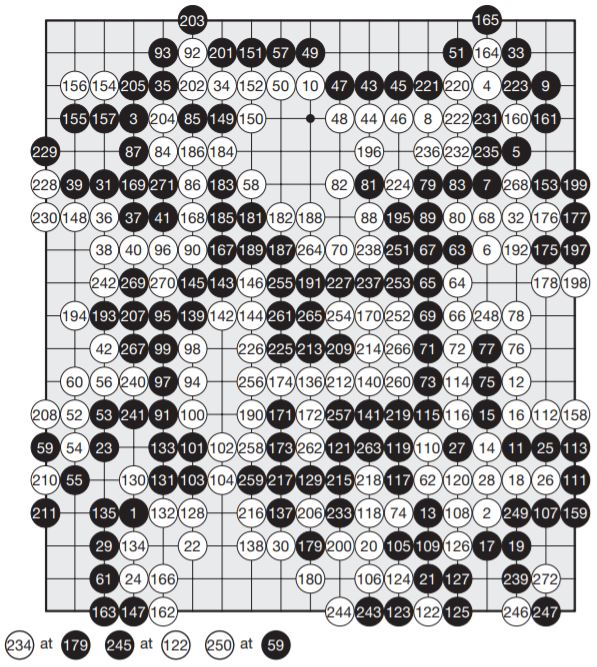
\includegraphics[width = 0.6\columnwidth]{Go_3}
    \caption{Fan Hui (Black), AlphaGo (White), AlphaGo wins by 2.5 points\cite{b12}}
    \label{Go_1}
\end{figure}

Combinatorial games have several ways of measuring game complexity,\cite{b3,b16}. Most widely used are \textit{state-space} complexity and \textit{game-tree} complexity (our main focus). The state-space complexity is defined as the number of legal game positions reachable from the initial position of the game. Whereas game-tree complexity is the total number of possible games that can be played; the total number of all possible reachable leaf nodes (end of the game) from the game's root node (initial position). Game-tree complexity may be larger than the state-space complexity, as the same position may occur at several different places in the game tree. Calculating the exact game-tree complexity of games such as chess is infeasible. Therefore, using tournament games, we observe the average game length, i.e., depth $d$, and determine the average branching factor $b$, either as a constant or a function of depth. Finally, raising the average branching factor $b$ to the power of the average length $d$, i.e., $b^d$, gives us an approximation. So, in large games, such as chess, we have $b \approx 35$ and $d \approx 80$, and Go has $b \approx 250$ and $d \approx 150$\cite{b4}. Thus an enormous game-tree complexity of $250^{150}$ (more than the number of atoms in the universe) for Go is intractable using brute force approaches.

\begin{figure}[t]
    \centering
    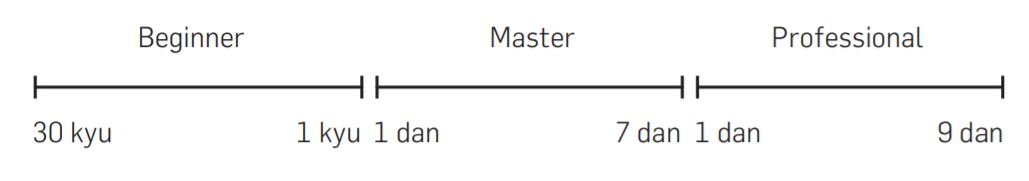
\includegraphics[width = \columnwidth]{Go_2}
    \caption{Ranking system in the game of Go\cite{b11}}
    \label{Go_ranking}
\end{figure}

\subsection{Deep Reinforcement Learning} \label{GT}
A wide variety of tasks in AI and optimal control can be formalized as sequential decision-making processes. Reinforcement learning (RL) is the study of approximating optimal decision-making in natural and artificial systems. Reinforcement learning can be subdivided into two fundamental problems: \textit{learning} and \textit{planning}\cite{b1}. We refer to the decision-making entity as the \textit{agent}, and everything outside of the \textit{agent} as its \textit{environment}. The goal of learning is for an agent to improve its \textit{policy} from its interactions with the environment. The goal of planning is for an agent to improve its policy without further interaction with the environment. Despite being different, these two problems are intimately related. During learning, the agent interacts with the environment by executing actions and observing their consequences. During planning, the agent can interact with a model of the environment by simulating actions and observing their consequences. At each time-step $t$, the agent receives observations $s_t \in S$ from its environment and executes an action $a_t \in A$ according to its behavior policy. The environment then provides a feedback signal in the form of a reward $r_{t+1} \in R$. This time series of actions, observations, and rewards defines the agent's \textit{experience}. In both cases (planning and learning), the agent updates its policy from its experience. The goal of RL is to improve the agent's future reward given its past experience\cite{b2}. 

The RL problem is deeply indebted to the idea of Markov decision processes (MDPs) from the field of optimal control. Since the game of Go is a classic combinatorial game (zero-sum, perfect information, deterministic, discrete, and sequential\cite{b17,b18}), it can be modeled as a fully observable finite MDP\cite{b2}. Most RL algorithms involve estimating \textit{value} functions -- functions of states (or of state-action pairs) that estimate how good is the agent's given state (or how good it is to perform a given action in a given state). The notion of `how good' is defined in terms of expected return that depends on the agent's action. Accordingly, value functions are defined with respect to the behavior, called policies. A \textit{policy}, $\pi(s_t, a_t)$ is a mapping from states to probabilities of selecting each legal action\cite{b2}. 

Solving RL problems means finding a policy that achieves maximum expected future rewards by selecting an optimal sequence of actions. For finite MDPs, there exists such an optimal policy. There may also exist more than one optimal policies but they share the same optimal state-value function, $v_*(s)$ (or optimal state-action value function, $q_*(s,a)$). A well-defined notion of optimality organizes the approach to \textit{learning} we described earlier. For the kind of task in which we were interested, developing an AI for Go, learning optimal policies can only be done with high computational cost and time. In tasks with small, finite state sets (such as tic-tac-toe), it is possible to form these approximations using tables with one entry for one state (or state-action pair). These we call the \textit{tabular} methods. In many cases of practical application, however, there are far more states (e.g., game-tree of Go) than could possibly be entries in a table. In these cases, the functions must be approximated using a more compact parameterized function representation. Thus our framing of the RL problem for the game of Go forces us to settle for approximations. That is where deep learning helps to approximate both policy and value functions. In particular, deep convolutional neural networks (DCNNs) are powerful at giving you higher-level representations of image data \cite{b19,b20}, and also accurately mimics predictions of a labelled data \cite{b21,b22,b23}. In AlphaGo, both policy and value functions are learned by reinforcement learning with function approximation provided by DCNNs. Hence the name deep reinforcement learning. It is worth noting that instead of deep reinforcement learning starting with randomly initialized weights, it started from weights learned from a large collection of human expert moves. More specifics on training these networks are discussed in Sec.~\ref{AlphaGo}.


% Decision theory (or planning) combines probability theory with utility theory to provide a formal and complete framework for decisions made under uncertainty. Game theory extends decision theory to situations in which multiple agents interact. A game can be defined as a set of established rules that allow the interaction of one or more players to produce specified outcomes. The following properties classify games: number of players involved, whether the reward to all players sums to zero (zero-sum), whether the state of the game is fully or partially observable to the players (information), whether uncertainty plays a part (determinism), whether actions are applied sequentially (sequential), and whether actions are discrete in real time (discrete). Games with two players that are zero-sum, perfect information, deterministic, discrete, and sequential are called combinatorial games (e.g., chess, Go). They have controlled environments defined by simple rules but typically exhibit deep and complex play, as amply demonstrated by Go.

% A Markov decision process (MDP) models RL problems in fully observable environments (like Go) using four components: $S$ (a set of states, with $s_0$ being the initial state), $A$ (a set of actions), $P(s,a,s')$ (a transition model determining the probability of reaching state $s'$ if action $a$ is applied to state $s$), and $R(s)$ (a reward function). Overall decisions are modeled as sequences of (state, action) pairs, in which a probability distribution decides the next state $s'$ given the current state $s$ and the chosen action $a$. In addition, the main objective is to find the policy $p$ that maps from states to actions, specifying which action will be chosen from each state $S$ that yields the highest expected reward.

% % Think about this section -- needs to be well built 
% Due to its generality, RL is studied in many disciplines, such as game theory, control theory, operations research, multi-agent systems, swarm intelligence, and statistics.\ RL is a computational approach to understanding and automating goal-directed learning (similar to sequential decision-making). RL uses the framework of MDP (Sec.~\ref{GT}) to define the interaction between a learning agent and its environment in terms of states, actions, and rewards. In this rich text of RL, there are two categories of solution methods: one caters to small and tractable state spaces, known as \textit{tabular} solution methods, the other caters to arbitrarily large state spaces (e.g., combinatorial games), known as \textit{approximate} solution methods. Deep reinforcement learning (DRL) algorithms incorporate deep learning to solve such intractable search space MDPs using policy gradient techniques of \textit{approximate} solution methods. DCNNs are powerful at giving you higher level representations of image data and also accurately mimics predictions of a labelled data. In AlphaGo, many board positions as a 19 x 19 image are passed through architectures of two DCNNs (policy and value networks respectively) to construct offline knowledge of the game of Go. More specifics on training these networks is discussed in Sec.~\ref{AlphaGo}.



\subsection{Monte Carlo tree-search} \label{MCTS_basic}
Monte Carlo methods (MCM) have their roots in statistical physics, where they have been used to obtain approximations to intractable integrals\cite{b24}, and have since been used in a wide array of domains. MCMs rely on repeated random sampling to obtain numerical results. The key idea is to use randomness to solve problems that might be deterministic in principle. Thus MCMs were applied to solve RL problems based on averaging sample rewards, nowadays heavily in games AI research \cite{b18,b25}. Monte Carlo tree search (MCTS) rests on two fundamental concepts of MCMs: the actual value of action may be approximated using random simulation, and these values may be used efficiently to adjust the policy towards a best-first action strategy \cite{b18}. The algorithm progressively builds a partial game tree, guided by the previous tree exploration. The tree is used to estimate the values of actions, with these estimates (particularly those most promising actions) becoming more accurate as the tree is built.

The basic algorithm works iteratively, building a search tree until a computational budget, typically time, memory, or iteration constraint, is reached. Then the search stops, and the best performing root action is returned. Each node in the search tree represents a state of the domain, and directed links to child nodes represent actions leading to subsequent states. Typical four steps (cf. Fig.~\ref{basic_MCTS}) applied per search iteration are:
\subsubsection*{Selection} Starting at root node, \textit{tree policy} is recursively applied to select optimal child nodes until a leaf node is reached. The leaf node is expandable if it represents a nonterminal state and has unexpanded and unvisited children.
\subsubsection*{Expansion} Expand the leaf node according to the available legal actions and choose one of its children. 
\subsubsection*{Simulation} Play a simulated game starting with that node according to a \textit{default policy} to produce an outcome. Sometimes this step is termed as \textit{evaluation}. 
\subsubsection*{Backpropagation} Use the results of that simulated game to update the node and its ancestors (till the root node). The simulation result is thus `backed up' (backpropagated). It does not use any policy but updates node statistics that inform future tree policy decisions. 

\begin{figure}[t]
\centerline{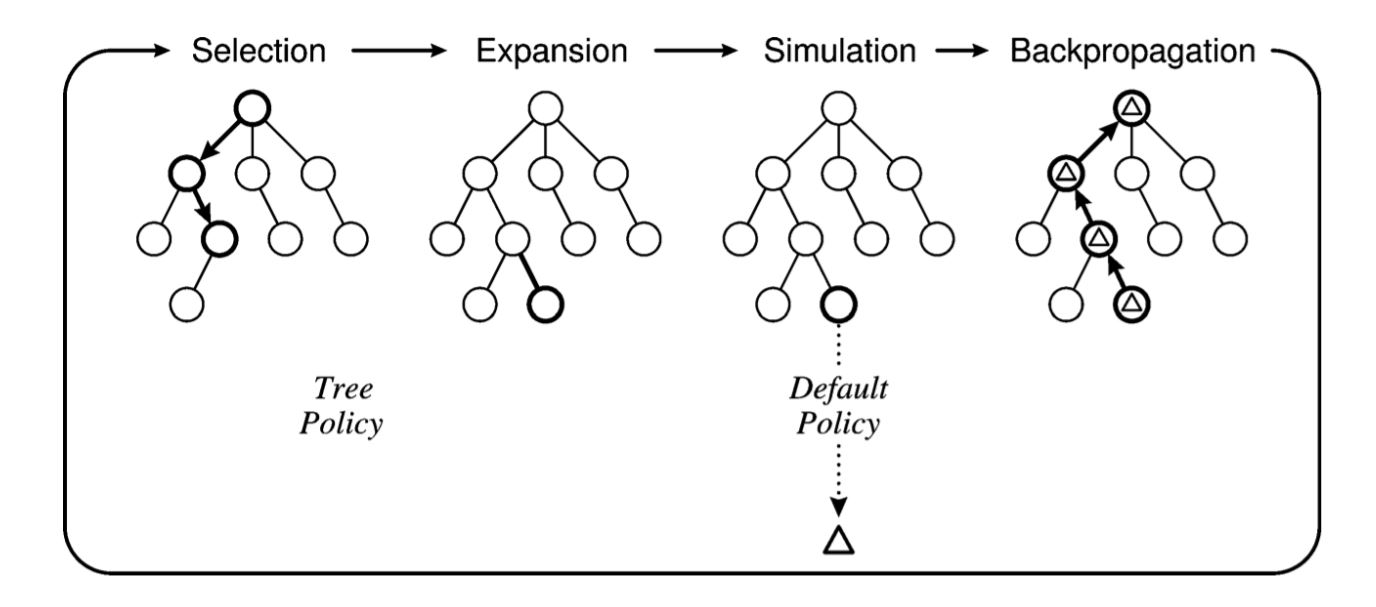
\includegraphics[width = 0.8\columnwidth]{Basic_MCTS.JPG}}
\caption{One iteration of the basic Monte Carlo tree search\cite{b18}}
\label{basic_MCTS}
\end{figure}


\section{AlphaGO} \label{AlphaGo}
This section describes the main innovation that made AlphaGo a strong Go player. First, it builds an offline knowledge representation of the game of Go using DCNNs trained through several steps of its machine learning pipeline (cf. Fig~\ref{ML_pipe_1}). Second, it efficiently combines these networks with asynchronous policy and value MCTS (APV-MCTS) to select final moves during real-time plays. 


\subsection{Supervised learning of policy network}
In the first stage in our offline training, to initialize the weights for reinforcement learning of the policy network, a 13-layer supervised learning (SL) policy network was trained using a randomly sampled dataset (state-action pairs) from 30 million expert human moves (KGS Go Server). The SL policy network $p_\sigma(a|s)$ takes an input $s$ (Extended Table 2 in\cite{b12}), alternates between convolutional layers and rectifier nonlinearities, and outputs a probability distribution over all legal moves $a$ using a final softmax layer. The policy network was trained using stochastic gradient ascent to maximize the likelihood of the human move $a$ selected in state $s$,
\begin{equation}
    \nabla \sigma \propto \frac{\partial \log p_\sigma (a|s)}{\partial \sigma}.
\end{equation}
The network predicted expert moves on a held-out test set with an accuracy of 57.0\% using all input features and 55.7\% using only raw board position and move history as inputs. Minor improvements in accuracy led to significant improvements in playing strength (cf. Fig.~\ref{SL_strength}); more extensive networks achieve better accuracy but are slower to evaluate during search (see Extended Table 3 in\cite{b12} for accuracies of these networks).

\begin{figure}[t]
\centerline{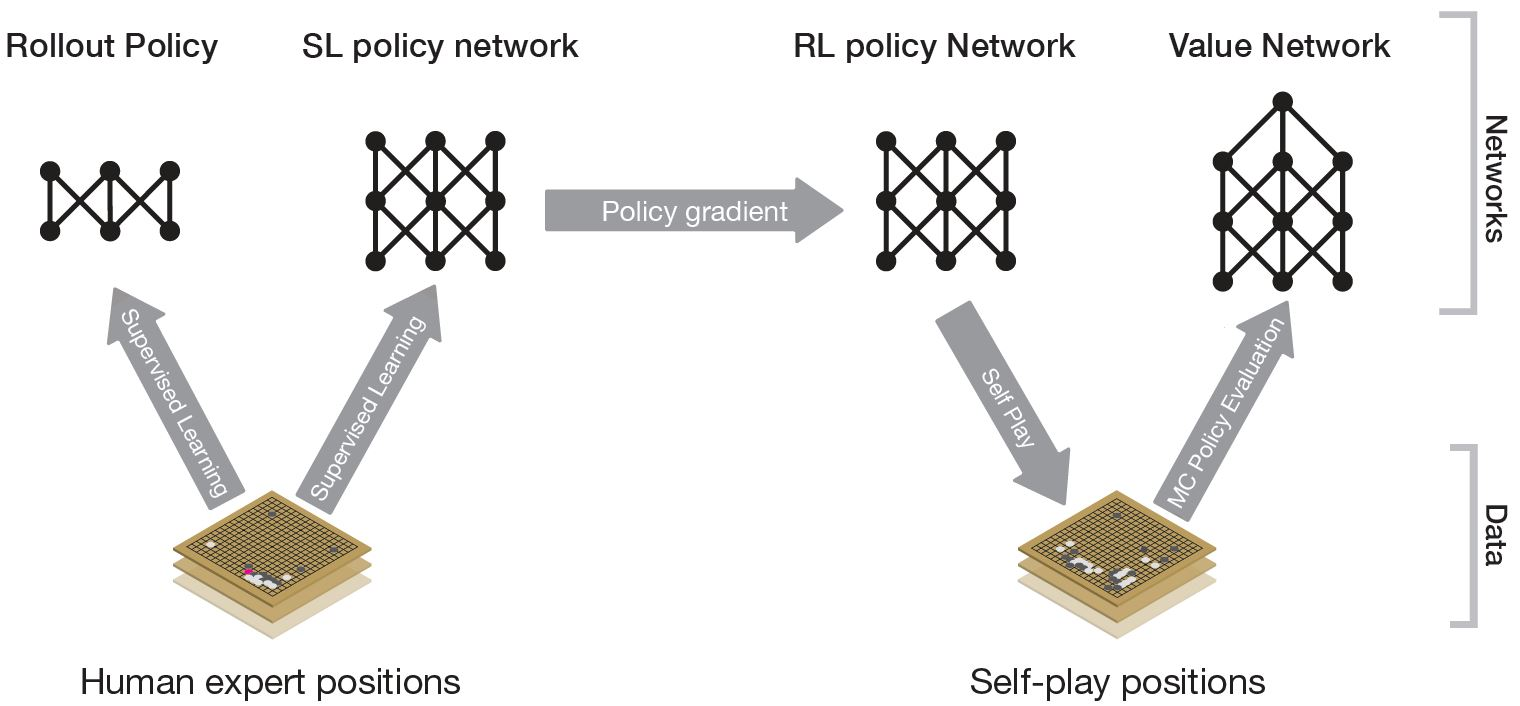
\includegraphics[width = \columnwidth]{ML_pipeline_3.jpg}}
\caption{Machine learning training pipeline of AlphaGo\cite{b12}}
\label{ML_pipe_1}
\end{figure} 

\begin{figure}[b]
\centerline{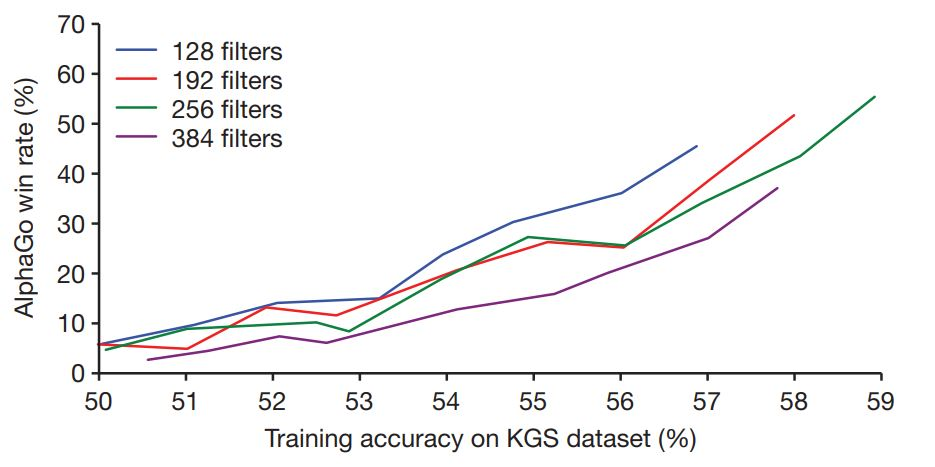
\includegraphics[width = 0.8\columnwidth]{Sl_strength.JPG}}
\caption{Strength of supervised learning policy network\cite{b12}}
\label{SL_strength}
\end{figure}


% \begin{figure*}[t]
% \centerline{\includegraphics[width = 5in]{ML_pipeline_2.jpg}}
% \caption{Offline machine learning training pipeline of AlphaGo}
% \label{ML_pipe}
% \end{figure*}

% \begin{table*}[]
%     \centering
%     \begin{tabular}{c|c}
%          &  \\
%          & 
%     \end{tabular}
%     \caption{Caption}
%     \label{tab:my_label}
% \end{table*}


\subsection{Rollout policy network}
Although the largest SL policy networks achieved the highest accuracy, a faster policy network was needed to simulate the games of self-play. Hence, a rollout policy, $p_\pi$, which uses a more simple linear softmax classifier on small pattern features, was developed (Extended Table 4 in \cite{b12}). It takes 2$\mu$s to compute each move instead of the 3ms with the SL policy network. This rollout policy has an accuracy of 24.2\% (compared to 55.7\%), but it is 1500 times faster. 


\subsection{Reinforcement learning of policy network} \label{RL_pn}
The second stage of offline training was to go further than just mimicking expert human moves. Silver et al.\cite{b12} wanted AlphaGo to learn new, improved policies on its own. Policy gradient RL techniques were applied to the SL policy network to get an improved reinforcement learning (RL) policy network, $p_\rho$ (identical in structure to SL policy network). In RL literature, they are termed ubiquitously as \textit{behavior policy} and \textit{target policy}. The new, improved policy being learned is called the target policy (in our case, RL policy), and the policy used to generate behavior is called the behavior policy (in our case, SL policy). The weights of the RL policy network were first initialized as $\rho = \sigma$. Next, games were played using the new RL policy network against randomly selected from the set of older RL policy networks. Games were not played with the same policy network to avoid overfitting the current policy (i.e., it will memorize the moves rather than generalize them for different opponents). The game is played till the terminal state. A reward function $r(s)$ that is zero for all non-terminal time steps $t<T$ was used. The outcome $z_t = \pm r(s_T)$ is the terminal reward at the end of the game from the perspective of the current player at time step t: $+1$ for winning and $-1$ for losing. The weights of the RL policy network are updated similarly to the SL policy network, except we use the game result $z_t$ to determine which direction to move in the stochastic gradient ascent that maximizes this expected outcome $z_t$,
\begin{equation}
    \nabla \rho \propto \frac{\partial \log p_\rho (a_t|s_t)}{\partial \rho}z_t.
\end{equation}

\begin{figure}[b]
\centerline{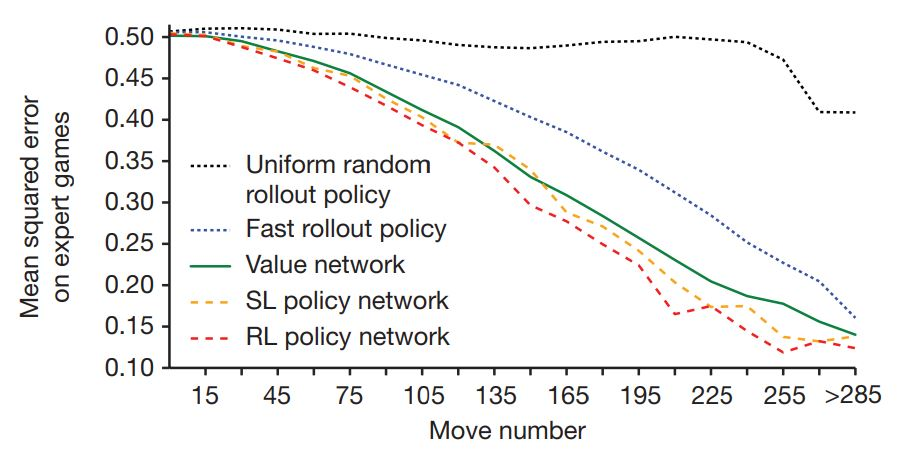
\includegraphics[width = 0.8\columnwidth]{RL_acc.JPG}}
\caption{Accuracy of reinforcement learning value network\cite{b12}}
\label{RL_accu}
\end{figure}


\subsection{Reinforcement learning of value network}
The final stage of our offline training was estimating a value function $v_p(s)$ that predicts the outcome from position $s$ of games played by using policy $p$ for both players. The goal is to converge to an optimal value function, $v^*(s)$, under perfect play. Silver et al.\cite{b12} estimated the value function $v^{p_\rho}(s)$ for the strongest RL policy network $p_\rho$. The value function was approximated using a value network $v_\theta(s)$ with weights $\theta$, 
% $v_\theta(s) \approx v^{p_\rho}(s) \approx v^*(s)$
\begin{equation}
   v_\theta(s) \approx v^{P_\rho}(s) = E[z_t\ |\ s_t = s, a_{t...T} \sim p] \approx v^*(s).
\end{equation}

This neural network has a similar architecture to the policy network but outputs a single prediction instead of a probability distribution. To train this network, we use the outcomes of the self-play games, $z$, from Sec.~\ref{RL_pn}. From the start to the finish of a game, many board positions from the move sequence can be added to the training dataset, but not more than one board position per game is collected. All board positions in the same game lead to the same result (a win or a loss); they are strongly correlated. To train a model effectively, samples in the training dataset need to be independent. Therefore, we use the RL policy network to play more than 30 million games and collect only one position from each game into the training dataset. We train the weights by regression on these state-outcome pairs $(s, z)$, using stochastic gradient descent to minimize the mean squared error (MSE) between the predicted value $v_\theta(s)$, and the corresponding outcome $z$,
\begin{equation}
    \nabla \theta \propto \frac{\partial v_\theta(s)}{\partial \theta} (z - v_\theta(s)).
\end{equation}
Training on this data set led to MSEs of 0.226 and 0.234 on the training and test set, respectively, indicating minimal overfitting. Fig.~\ref{RL_accu} shows the position evaluation accuracy of the value network, compared to Monte Carlo rollout outcomes using the fast rollout policy $p_\pi$; the value function was consistently more accurate. A single evaluation of $v_\theta(s)$ also approached the accuracy of Monte Carlo rollouts using the RL policy network $p_\rho$ but using 15,000 times less computation.

\begin{figure}[t]
\centerline{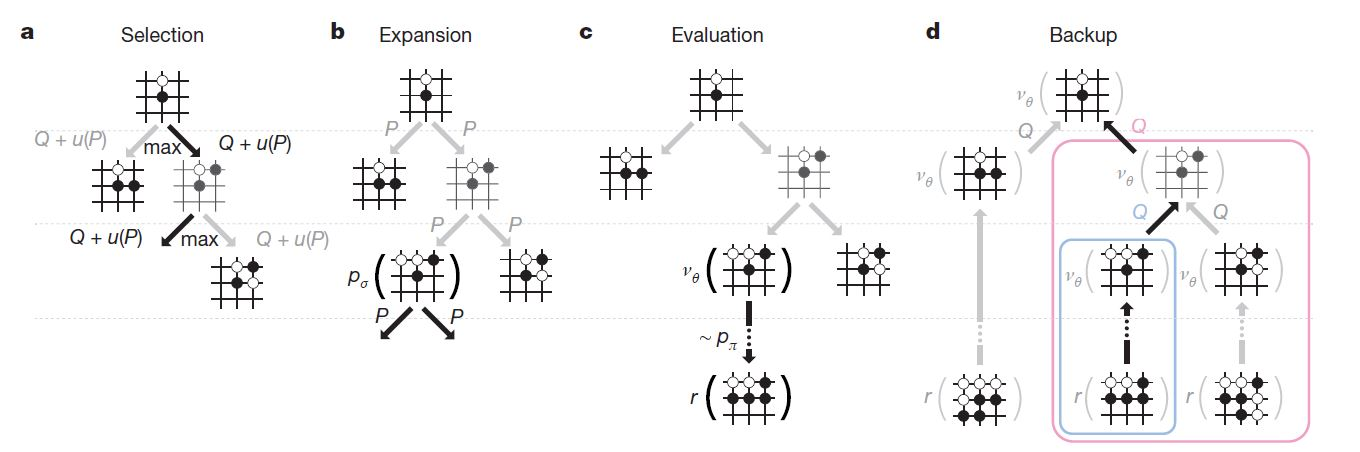
\includegraphics[width = \columnwidth]{MCTS.JPG}}
\caption{Monte Carlo tree-search in AlphaGO\cite{b12}}
\label{MCTS_1}
\end{figure}

\subsection{APV-MCTS search algorithm}\label{MCTS}
% So what did they achieve so far? The training is done and they have a policy network that tells us what moves are promising at a given board position, and a value network that tells us how good is a board position.
The last task was to combine the offline knowledge of both networks with the online knowledge of APV-MCTS, like in\cite{b26}. Let us assume our search tree looks like the one in the \textit{selection} step (cf. Fig.~\ref{MCTS_1}). Each edge $(s, a)$ represents an action $a$ to transit from state $s$ to state $s'$. Each edge stores a set of statistics, $\{ P(s,a), W_v(s,a),$ $W_r(s,a), N_v(s,a), N_r(s,a), Q(s,a)\}$, where $P(s,a)$ is the prior probability, $W_v(s,a)$ and $W_r(s,a)$ are Monte Carlo estimates of total action value, accumulated over $N_v(s,a)$ and $N_r(s,a)$ leaf evaluations and rollout rewards respectively, and $Q(s,a)$ is the combined mean action value for that edge. The APV-MCTS follows the four basic steps outlined in Fig.~\ref{MCTS_1}.

\subsubsection*{Selection} The purpose of this step is to prioritize moves for further simulations. At each time step $t$ of each simulation, starting from the root node, the game-tree is traversed until a leaf node is reached at time step L. At each of $t<L$, an action $a_t$ is selected from state $s_t$ such that,
\begin{equation}\label{sel_leaf}
    a_t = \arg\max_a( Q(s_t,a) + u(s_t,a)),
\end{equation}
 using a variant of PUCT algorithm\cite{b27, b28}. The bonus term $u(s,a) = c_{puct} P(s,a) \frac{\sqrt{\sum_b N_r(s,b)}}{1+N_r(s,a)}$ is proportional to the prior probability $P(s,a) = p_\sigma(a|s)$ ($p_\sigma$ is the SL policy network) and $c_{puct}$ (a constant that determines the level of exploration), and inversely to $1+N_r(s,a)$. Initially the traversal to the best leaf node prefers actions with high probability and low visit counts, but asymptotically prefers action with high action value, $Q(s,a)$, which is calculated from the backpropagation of the previously simulated game results. Using \eqref{sel_leaf}, the partial game tree is traversed (highlighted in black in Fig.~\ref{MCTS_1}a) to a leaf node $s_L$ at step length $L$, which maybe expanded.
 
 Before we see how a leaf node may be expanded, it is better to see how it is evaluated and its results backpropagated to the root node. This essentially helps us understand which leaf nodes to focus on and expand further.

\subsubsection*{Evaluation and Backup}
The leaf node $s_L$ is added to the queue for evaluation $v_\theta(s_L)$ by the value network (unless previously evaluated). Next, at each time step $t \geq L$, a game is simulated from $s_L$ by sampling actions using the rollout policy $a_t \sim p_\pi(\cdot | s_t)$ (for both players) until the end of the game. 
% It means finish playing a game using a policy and find out whether you win or loss. 
When the game reaches a terminal state, the outcome $z_L = \pm r(s_T)$ is computed. 
% So a final leaf evaluation $V(s_L)$ is calculated by combining the evaluation by the value network $v_\theta(s_L)$ with the outcome $z_L$ using a mixing parameter $\lambda$. 
% So the leaf node $s_L$ is evaluated in two steps: first, by the value network $v_\theta(s_L)$; and second, by the outcome $z_L$ of a random rollout played out until terminal step $T$ using the fast rollout policy $p_\pi$; these evaluations are combined, using a mixing parameter $\lambda$ to get a final leaf evaluation $V(s_L)$.
% \begin{equation}
%     V(s_L) = (1 - \lambda)v_\theta(s_L) + \lambda z_L
% \end{equation}
% \subsubsection{Backup}
Next, at each step $t \leq L$ of that simulation, the rollout statistics are updated as if it has lost $n_{vl}$ games (parameter used to discourage other threads in multi-machine simulation\cite{b28}), $N_r(s_t, a_t) := N_r(s_t, a_t) + n_{vl}$; $W_r(s_t, a_t) := W_r(s_t, a_t) - n_{vl}$. At the end of the simulation, the rollout statistics are updated in the first backward pass through each step $t \leq L$, replacing the virtual losses by the outcome, $N_r(s_t, a_t) := N_r(s_t, a_t) - n_{vl} + 1$; $W_r(s_t, a_t) := W_r(s_t, a_t) + n_{vl} + z_t$. Asynchronously, a separate backward pass is initiated when the evaluation of the leaf position $v_\theta(s_L)$ completes. The output $v_\theta(s_L)$ is used to update value statistics in a second backward pass through each step $t \leq L$, $N_v(s_t, a_t) := N_v(s_t, a_t) + 1$, $W_v(s_t, a_t) := W_v(s_t, a_t) + v_\theta(s_L)$. The overall evaluation of each state action is a weighted average of the Monte Carlo estimates, that mixes together the value network and rollout evaluations with a weighting parameter $\lambda$,
\begin{equation}
    Q(s,a) = (1 - \lambda)\frac{W_v(s,a)}{N_v(s,a)} + \lambda \frac{W_r(s,a)}{N_r(s,a)}.
\end{equation}


% At the end of simulation, the visit counts and action values of all traversed edges are updated. Each edge accumulates the visit count and mean action evaluation of all simulations passing through that edge
% \begin{align}
%     N(s,a) &= \sum_{i=1}^n1(s,a,i)\\
%     Q(s,a) &= \frac{1}{N(s,a)} \sum_{i=1}^n1(s,a,i)V(s_L^i)
% \end{align}
% where $s_l^i$ is the leaf node from the $i^{th}$ simulation, and $1(s, a, i)$ indicates
% whether an edge $(s, a)$ was traversed during the $i^{th}$ simulation. When a sufficiently large tree is traversed, the search is complete and the algorithm chooses the most visited move from the root position.

\subsubsection*{Expansion}When the visit count exceeds a threshold, $N_r(s, a) > n_{thr}$, the successor state $s'$ is added to the search tree. The new node is initialized to $\{ N(s',a) = N_r(s', a) = 0,\ W(s',a) = W_r(s',a) = 0,\ P(s',a) = p_\tau(a|s')\}$, using a tree policy $p_\tau(a|s')$ (similar to the rollout policy but with more features, see Extended Table 4 in \cite{b12}) to provide a placeholder prior probability. The position $s'$ is also inserted into a queue for asynchronous evaluation by the SL policy network. Prior probabilities are computed by the SL policy network $p_\sigma(\cdot |s')$ and these replace the placeholder prior probabilities, $P(s',a) := p_\sigma^\beta(a |s')$ (with a softmax temperature parameter set to $\beta$). You may ask why not use the RL policy network. Humans select a diverse beam of promising moves which is represented by the SL policy network $p_\sigma$. Hence, it performed better than the strongest RL policy network $p_\rho$ because RL optimizes for the single best move. At the end when the computational budget is reached, a sufficiently large tree-search is complete, and the algorithm chooses the most visited edge at the root node as the final move to play.

% Positions are
% evaluated by both the policy network and the value network using a mini-batch
% size of 1 to minimize end-to-end evaluation time

% The leaf node $s_L$ from the previous step is expanded for possible legal moves (here two in Fig.~\ref{MCTS_1}b). We initialize these new edges with $P(s,a) = p_\sigma(a|s),\ N(s,a) = 0,\ Q(s,a) = 0$. You may ask why it is not initiated by the RL policy network. Humans select a diverse beam of promising moves which is represented by the SL policy network $p_\sigma$. Hence, it performed better than the stronger RL policy network $p_\rho$ because RL optimizes for the single best move.


\section{Evaluation and analysis of AlphaGo}
This section describes how AlphaGo was evaluated with existing computer Go programs and human players. Further, it analyses the extent to which this new search technique has been applied in general computer game-playing.

\subsection{Against other Go programs and expert human Go players}
Before AlphaGo, several extensions of MCTS had led to high-performance Go programs; \textit{Pachi}\cite{b29} and \textit{Feugo}\cite{b30} were the strongest in the open-source community, and \textit{Zen} and \textit{Crazy Stone}\cite{b31} were likewise in the commercial domain. The performance of the RL policy network was first evaluated by playing against Pachi. In contrast to the ones only based on supervised learning of DCNNs\cite{b32, b33}, it won 85\% of games against Pachi and 80\% against the SL policy network. Next, AlphaGo was evaluated against all the above programs in an internal tournament, including an additional open-source program \textit{GnuGo}, based on state-of-the-art search methods that preceded MCTS (cf. Fig.~\ref{Eval_AplhaGo}a). Programs were evaluated on an Elo scale \cite{b34}. All were allowed 5s of computation time per move. AlphaGo turned out to be many dan ranks stronger, winning 494 out of 495 games (99.8\%) against any previous Go programs. Games with four handicap stones were also played to provide a fair challenge to AlphaGo, and it won 77\%, 86\%, and 99\% of handicap games against Crazy Stone, Zen, and Pachi, respectively. Silver et al.\cite{b12} also developed a distributed version that won 77\% of games against single-machine AlphaGo and 100\% against other programs. 
\begin{figure}[t]
    \centering
    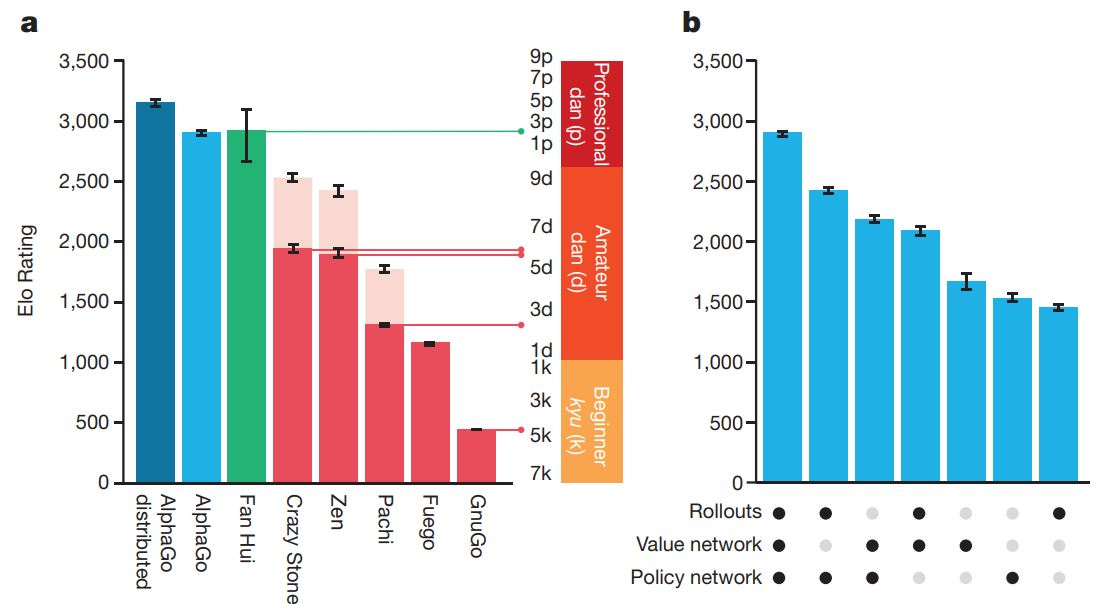
\includegraphics[width = 0.85\columnwidth]{Eval_1}
    \caption{Tournament evaluation of AlphaGo\cite{b12}}
    \label{Eval_AplhaGo}
\end{figure}
Other variants of AlphaGo (cf. Fig.~\ref{Eval_AplhaGo}b), e.g., using just the value network $(\lambda=0)$ exceeded the performance of all other Go programs, showing that value networks provide a viable alternative to Monte Carlo evaluation. However, the mixed version $(\lambda=0.5)$ performed best, winning $\geq$95\% of games against other variants. This combination of the two different position-evaluation methods is complementary: the value network approximates the outcome of games played by the strong but slow $p_\rho$, while the rollouts can precisely score and evaluate the outcome of games played by the weaker but faster rollout policy $p_\pi$.

% \subsection{Against expert human Go players}
AlphaGo (distributed version) was evaluated against three-time European Champion Mr. Fan Hui, a professional 2-dan Go player (in 2015). AlphaGo's win (5-0) was the first time a computer Go program defeated a human professional without a handicap. AlphaGo then competed against Mr. Lee Sedol, winner of 18 world titles (in 2016). AlphaGo's 4-1 victory was a landmark achievement a decade ahead of its time. AlphaGo thus earned a 9-dan professional ranking (highest rank), the first-ever accolade received by a computer Go program. In January 2017, an online version of AlphaGo called Master achieved 60 straight wins in time-control games against top international players. Four months later, Master took part in the Future of Go Summit in China, the birthplace of Go. Master defeated the Chinese grandmaster Mr. Ke Jie in a match (3-0). 

\subsection{AlphaGo family}
\subsubsection*{AlphaGo Zero} AlphaGo Zero\cite{b35} was developed after the Chinese Summit. While AlphaGo learned the game by playing thousands of matches with amateur and professional players, AlphaGo Zero learned by playing against itself (starting from completely random play). This powerful technique successfully accumulated thousands of years of human knowledge by training for just a few days. It quickly surpassed all previous versions' performance and discovered new knowledge, developing unconventional strategies and intuitive new moves. 

\subsubsection*{AlphaZero} AlphaZero\cite{b36} was introduced in late 2017. It mastered the games of chess, shogi, and Go by learning from scratch (beating a world-champion computer program in each case). It replaces hand-crafted heuristics with a deep neural network and algorithms that are given only the basic rules. 
% E.g., in its chess games, players saw that it had developed a highly dynamic and unconventional style that differed from any previous chess-playing engine.  

\subsubsection*{MuZero} MuZero\cite{b13} is the latest version of the AlphaGo family. It takes these ideas of AlphaZero one step further. It is a new approach to model-based RL. It achieves state-of-the-art performances in Atari 2600 games as well in chess, shogi, and Go, without prior knowledge of the game dynamics. It uses AlphaZero's powerful search and policy iteration algorithms and incorporates the learned model into the training procedure. It extends to a broader set of environments, including single-agent domains and non-zero rewards at intermediate time steps. It allows planning winning strategies in unknown domains, a significant leap forward in the capabilities of RL algorithms, and an essential step towards building general-purpose learning systems.  

\begin{figure}[t]
    \centering
    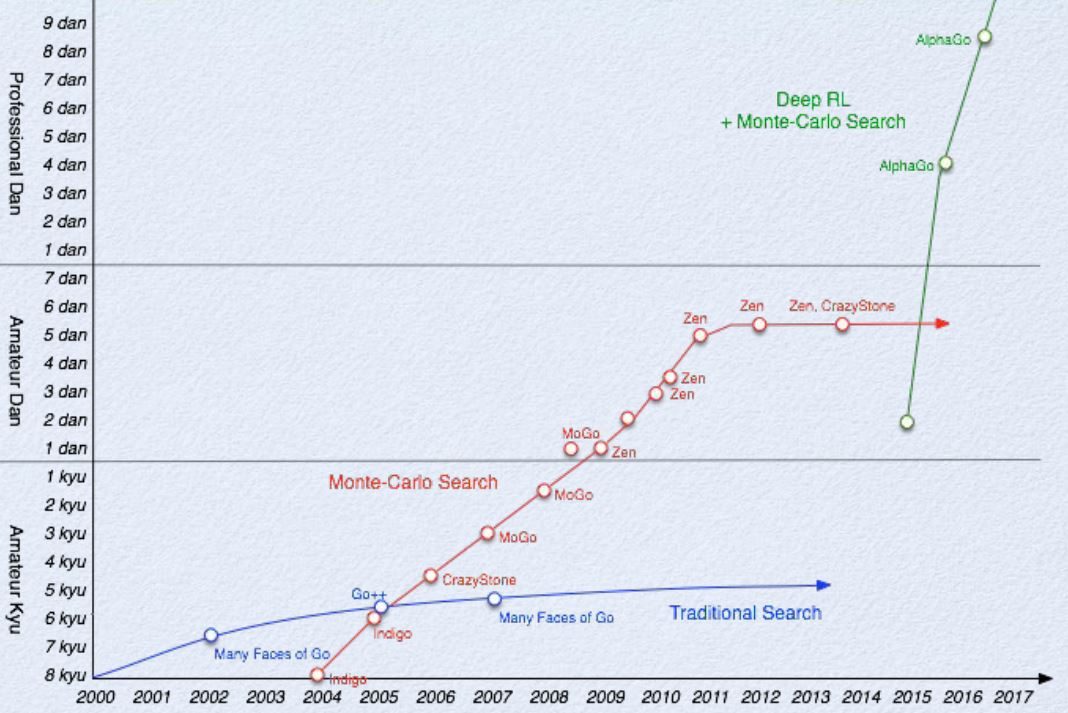
\includegraphics[width = 0.7\columnwidth]{Con_2.2}
    \caption{Progress in Computer Go\cite{b26}}
    \label{Prog_comp_go}
\end{figure}
 
\section{Conclusion and Outlook}
The game of Go epitomizes the challenges faced by many real-time sequential decision-making problems: an intractable search space, a significant branching factor, delayed consequences of actions, and a complex optimal solution infeasible to approximate using a policy or value function directly. MCTS is applied for planning in this challenging domain, which has proven to have implications well beyond the two-player games; for example, general game-playing, classical planning, partially observed planning, scheduling, and constraint satisfaction\cite{b11}. By combining MCTS with deep RL, AlphaGo took up the slack just when development in computer Go was thought to be stalled (cf. Fig.~\ref{Prog_comp_go}). It led to a spectacular performance taking us beyond amateur dan into the professional regime and ultimately beyond human capabilities. Research in further versions of AlphaGo has led to MuZero that needs no domain knowledge, no rules, and no human data. While in its early days, the ideas behind MuZero's robust planning and model-learning algorithms may pave the way towards tackling messy real-world RL problems where the “rules of the game” are unknown. 
% Moreover, this level of sophistication has helped us build confidence that such learning-based AI can be used as a positive multiplier for human ingenuity. 


\section*{Acknowledgment}
I gratefully acknowledge Dr.\ David Silver for sharing his presentation based on his paper ``Combining online and offline knowledge in UCT'' which received the Test of Time Award at ICML 2017 for my reference.


\begin{thebibliography}{}

\bibitem{b1} Silver, D., ``Reinforcement Learning and Simulation-Based Search in Computer Go,'' PhD thesis, Dept. of Computing Science, Univ. Alberta, Edmonton, Alberta, 2009.

\bibitem{b2} Sutton, R. \& Barto, A., ``Reinforcement Learning: an Introduction,'' MIT Press, 2018.

\bibitem{b3} Schaeffer, J., ``The game computers (and people) play,'' Advances in Computers, Volume 52, 189–266, 2000.

\bibitem{b4} Allis, L. V., ``Searching for Solutions in Games and Artificial Intelligence,'' PhD thesis,
Univ. Limburg, Maastricht, The Netherlands, 1994.

\bibitem{b5} Campbell, M., Hoane, A. \& Hsu, F., ``Deep Blue,'' Artificial Intelligence, Volume 134, 57–83, 2002.

\bibitem{b6} Schaeffer, J. et al., ''A world championship caliber checkers program,'' Artificial Intelligence, Volume 53, 273–289, 1992.

\bibitem{b7} Buro, M., ``From simple features to sophisticated evaluation functions,'' Computers and Games, Volume 1, 126–145, 1999.

\bibitem{b8} Tesauro, G., ``TD-gammon, a self-teaching backgammon program, achieves master-level play,'' Neural Computation, Volume 6, 215–219, 1994.

\bibitem{b9} Knuth, D. E. \& Moore, R. W., ``An analysis of alpha-beta pruning,'' Artificial Intelligence, Volume 6, 293–326, 1975. 

\bibitem{b10} Müller, M., ``Position evaluation in computer go,'' International Computer Games Association, Volume 25, 219-228, 2002.

\bibitem{b11} Gelly, S. et al., ``The grand challenge of computer Go: Monte Carlo tree search and extensions,'' Communications of the ACM, Volume 55, 106–113, 2012.

\bibitem{b12} Silver, D., Huang, A., Maddison, C. et al., ``Mastering the game of Go with deep neural networks and tree search,'' Nature, Volume 529, 484–489, 2016.

\bibitem{b13} Schrittwieser, J., Antonoglou, I., Hubert, T. et al., ``Mastering Atari, Go, chess and shogi by planning with a learned model,'' Nature, Volume 588, 604–609, 2020.
 
\bibitem{b14} Müller, M.,``Computer Go,''Artificial Intelligence,Volume 134, 145-179, 2002.

\bibitem{b15} Van der Werf, E.C.D., ``AI techniques for the game of Go," PhD thesis, Universiteit Maastricht, The Netherlands, 2005.

\bibitem{b16} H. Jaap van den Herik, Jos W. H. M. Uiterwijk \& Jack van Rijswijck, ``Games solved: Now and in the future,'' Artificial Intelligence, Volume 134, Issues 1–2, 2002.

\bibitem{b17} Littman, M. L., ``Markov games as a framework for multi-agent reinforcement learning,'' In 11th International Conference on Machine Learning, 157–163, 1994.

\bibitem{b18} Browne, C. et al., ``A survey of Monte-Carlo tree search methods,'' IEEE Transactions on Computational Intelligence and AI in Games, Volume 4, 1–43, 2012.

\bibitem{b19} Krizhevsky, A., Sutskever, I. \& Hinton, G. E., ``ImageNet classification with deep convolutional neural networks.'' In Advances in Neural Information Processing Systems, 1097–1105, 2012. 

\bibitem{b20}Lawrence, S., Giles, C. L., Tsoi, A. C. \& Back, A. D., ``Face recognition: a convolutional neural-network approach,'' IEEE Transactions on Neural Networks and Learning Systems, Volume 8, 98–113, 1997.

\bibitem{b21} LeCun, Y., Bengio, Y. \& Hinton, G.E., ``Deep learning,'' Nature, Volume 521, 436–444, 2015.

\bibitem{b22} LeCun, Y., Bottou, L., Bengio, Y., \& Haffner, P., ``Gradient based learning applied to document recognition,'' Proceedings of the IEEE 86(11): 2278-2324, 1998.

\bibitem{b23} LeCun, Y. et al., ``Handwritten digit recognition with a back-propagation network," Advances in Neural Information Processing Systems, Volume 2, 1989.

\bibitem{b24} Metropolis, N., ``The Beginning of the Monte Carlo method,'' Los Alamos Science, Special Issue, 1987.

\bibitem{b25} Chaslot G., Bakkes S., Szita I., \& Spronck P., ``Monte-carlo tree search: a new framework for game AI,'' Artificial Intelligence and Interactive Digital Entertainment, AAAI Press, 216–217, 2008.

\bibitem{b26} Gelly, S., \& Silver, D., ``Combining Online and Offline Knowledge in UCT,'' International Conference of Machine Learning, 2007.

\bibitem{b27} Rosin, C.D., ``Multi-armed bandits with episode context,'' Annals of Mathematics and Artificial Intelligence, Volume 61, 203–230 2011.

\bibitem{b28} Segal, R. B., ``On the scalability of parallel UCT,'' Computers and Games, 36–47, 2011.

\bibitem{b29} Baudiš, P. \& Gailly, J.-L., ``Pachi: State of the art open source Go program,'' Advances in Computer Games, 24–38, Springer 2012.

\bibitem{b30} Müller, M., Enzenberger, M., Arneson, B. \& Segal, R., ``Fuego – an open-source framework for board games and Go engine based on Monte-Carlo tree search,''
IEEE Transactions on Computational Intelligence and AI in Games, Volume 2, 259–270, 2010.

\bibitem{b31} Coulom, R., ``Computing Elo ratings of move patterns in the game of Go,'' International Computer Games Association Journal, Volume 30, 198–208, 2007.

\bibitem{b32} Maddison, C. J., Huang, A., Sutskever, I. \& Silver, D., ``Move evaluation in Go using deep convolutional neural networks,'' 3rd International Conference on Learning
Representations, 2015.

\bibitem{b33} Clark, C. \& Storkey, A. J., ``Training deep convolutional neural networks to play go,'' International Conference on Machine Learning, 1766–1774, 2015.

\bibitem{b34} Coulom, R., ``Whole-history rating: a Bayesian rating system for players of time-varying strength,'' International Conference on Computers and Games, 2008.

\bibitem{b35} Silver, D., Schrittwieser, J., Simonyan, K. et al., ``Mastering the game of Go without human knowledge,'' Nature, Volume 550, 354–359, 2017.

\bibitem{b36} Silver D., Hubert T., Schrittwieser, J. et al., ``A general reinforcement learning algorithm that masters chess, shogi, and Go through self-play,'' Science, Volume 362, 1140-1144, 2018.

\end{thebibliography}


\end{document}

